\documentclass[a4j]{cis-resume}
\usepackage{amssymb}
\usepackage{graphicx}
\usepackage{float}

% ------------------------------------------------------------------------
% タイトル等の設定
% ------------------------------------------------------------------------
\title{歩行時における足の接地推定} % 発表タイトル
\author{鈴木 健太} % 発表者氏名
\course{情報システムコース} % 情報工学コース or 情報システムコース
\stunum{S163043} % 学生番号
\supervisor{平川 正人 教授} % 指導教員氏名&職階

\begin{document}
\maketitle

% ------------------------------------------------------------------------
% 行間の設定
%   どうしてもページ内に収まらない場合はここをいじる。
%   デフォルト値は0.85(clsファイルで規定)
% ------------------------------------------------------------------------
%\renewcommand{\baselinestretch}{0.8}


% ------------------------------------------------------------------------
% ここから本文スタート
% ------------------------------------------------------------------------

% ------------------------------------------------------------------------
% 情報システムコースの学生は,下記のコメントアウトを解除し,英語150ワード
% 程度の概要を記載.
% ------------------------------------------------------------------------
\section*{概要}
Measurement and analysis of human movements are applied to various fields such as kinematics and human-computer interface. In the field of human motion analysis, Analysis of walking motion: Gait analysis is one of the most attractive research topics. Gait analysis can be useful for estimation of human body composition, personal identification, training and rehabilitation, fall prevention, etc. When performing gait analysis, certain parameters related to the object are measured. This parameter is roughly divided into the following two. One is a spatial parameter. This includes step length, slide length, etc. One is a temporal parameter. This is a parameter that classifies each time zone by focusing on the position of the foot in one cycle of walking such as stance phase and swing phase.

In this study, we use PoseNet, one of the pose estimation libraries, to analyze the value of each keypoints during walking and extract the double legs supporting phase in a non-invasive manner. In experiments, it was shown that Fourier analysis could be used to extract the double legs supporting phase from information obtained from posture estimation.

\section{はじめに} \label{sec:introduction}
人の動作の計測,解析は運動力学やヒューマンコンピュータインターフェースなど様々な分野に応用されている.特に,人の動作の中でも歩容解析は,最も注目されている研究テーマの一つである.体組成の推定\cite{cite1},個人識別,トレーニングやリハビリテーション,転倒予防などに歩容解析が役立てることができる.歩容解析を行う上で,対象に関するあるパラメータを測定する.このパラメータは大きく分けて次の2つである.1つは空間的パラメータである.これはステップ長,スライド長などが含まれる.1つは時間的パラメータである.これは立脚期,遊脚期\cite{cite2}など歩行の1周期の中の足の位置に着目し各時間帯を分類したパラメータである.

本研究では,姿勢推定ライブラリの1つであるPoseNetを用いて,
歩行時における各特徴点の値を解析し非侵襲で両脚支持相を抽出することを目指す.実験では,フーリエ解析を用い,姿勢推定から得られた情報で両脚支持相を抽出できる可能性を示した.
\section{研究内容} \label{sec:details}
\subsection{データ収集}
対象が1人であり,自然な歩行を足全体が写るように横方向から撮影した.
この映像に対し,PoseNetを用い姿勢推定を行い手首,膝,足首の左右計6箇所の特徴点からデータを収集した.サンプリングは約$28\,\mathrm{hz}$で,特徴点の画素の位置よりそれぞれ左右の手首,膝,足首について行われた.PoseNetの仕様上,下半身の特徴点は左右の臀部,膝,足首である.今回の研究では,歩行時に大きく動く膝,足首,手首の特徴点を抽出した.
\subsection{フーリエ解析}
収集した特徴点に対して左右間の距離$l_i$を求めた.そして,$l_i$それぞれに対しフーリエ変換を行い,歩行周期も考慮し周波数成分の分析を行った.分析の結果が図\ref{fig:変換}である.図\ref{fig:変換}より,膝間の距離は$1.30\,\mathrm{hz} \fallingdotseq 0.77\,\mathrm{s}$の周期が,足首間の距離は$1.52\,\mathrm{hz} \fallingdotseq 0.66\,\mathrm{s}$が強く見られることがわかる.実際の歩行周期は目視で測定し,周波数$1.47\,\mathrm{hz}$,周期$0.68\,\mathrm{s}$であった.

\begin{figure}[H]
  \begin{flushleft}
  \vspace{15mm}
  \begin{tabular}{c}
    % ----------------------
    \begin{minipage}{0.3\linewidth}
      \begin{flushleft}
        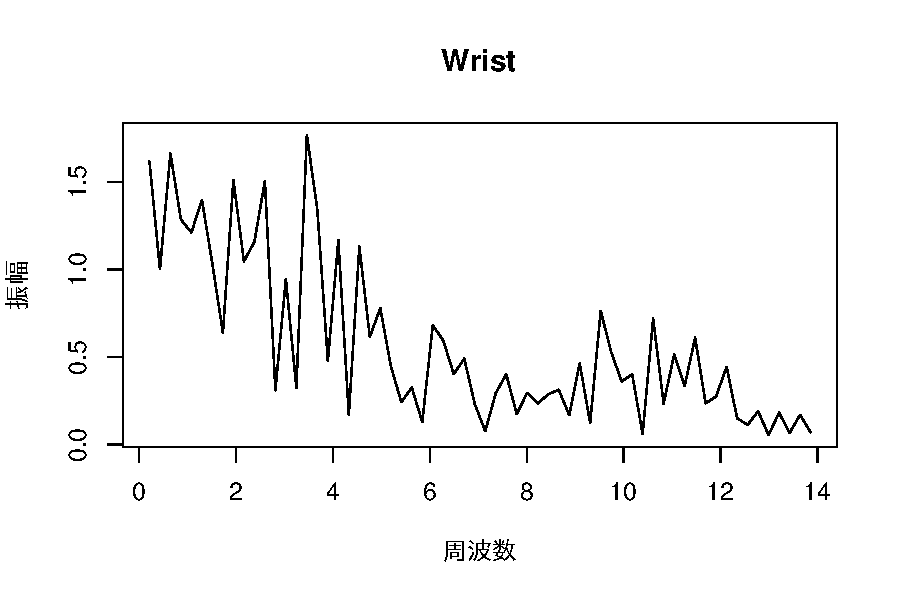
\includegraphics[keepaspectration,scale=0.3\figscale,angle=0]{Wrist.pdf}
      \end{flushleft}
    \end{minipage}
    % ----------------------
    \begin{minipage}{0.1\linewidth}
      \hspace{2mm}
    \end{minipage}
    % ----------------------
    \begin{minipage}{0.3\linewidth}
      \begin{center}
        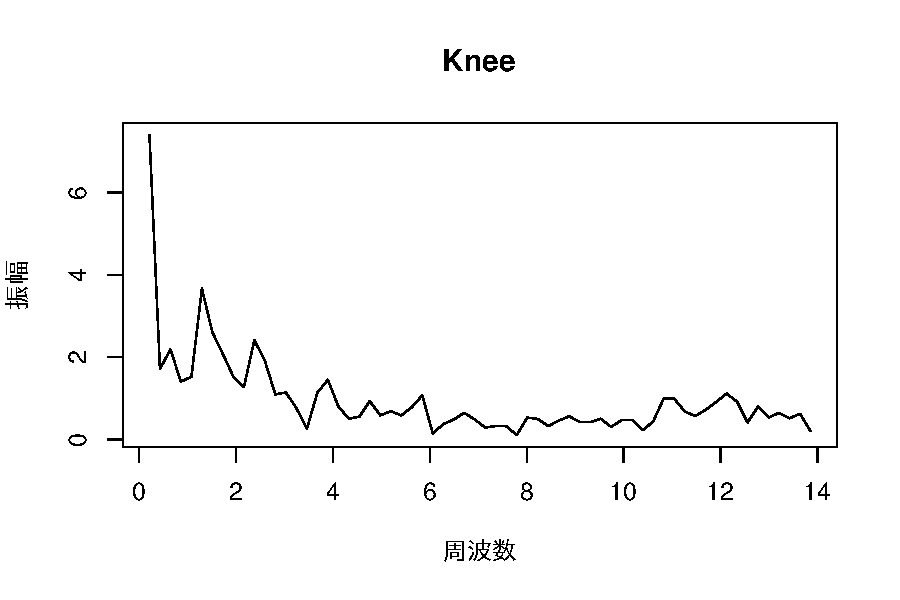
\includegraphics[keepaspectration,scale=0.3\figscale,angle=0]{Knee.pdf}
      \end{center}
    \end{minipage}
  \end{tabular}
    % ----------------------
    % \begin{minipage}{0.1\linewidth}
      \vspace{18mm}
    % \end{minipage}
    % ----------------------
    % \begin{minipage}{0.3\linewidth}
      \begin{flushleft}
        \hspace{1mm}
        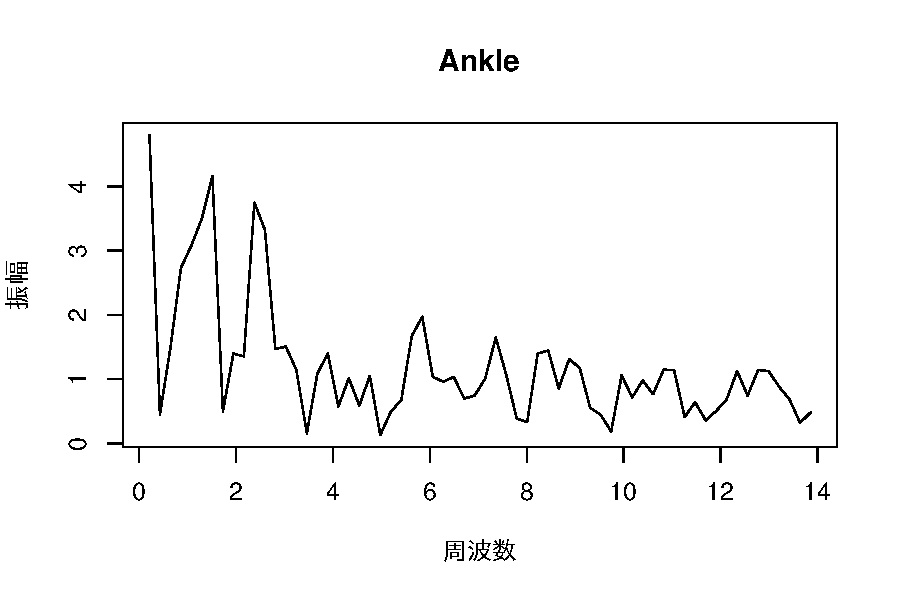
\includegraphics[keepaspectration,scale=0.3\figscale,angle=0]{Ankle.pdf}
      \end{flushleft}
    % \end{minipage}
  \caption{スペクトル} \label{fig:変換}
\end{flushleft}
\end{figure}
\subsection{解析結果の評価}
表\ref{tab:結果}より解析結果の歩行周期と目視で確認した周期との誤差率$\delta =|(\nu_i-\nu_t)/\nu_t|\times100\%$は,膝間の距離を解析したものが$11.72\%$,足首間の距離を解析したものが$3.00\%$である.よって,足首を見た場合がより実際の歩行周期に合っていることがわかった.また,推定された周期の山と谷の時間で歩行映像から切り取ったところ,両脚支持相を抽出できていることが確認できた.
\begin{table}[H]
  \caption{解析結果} \label{tab:結果}
  \begin{tabular}{c||ccc}
    \hline
            & 膝 $\nu_1$    & 足首 $\nu_2$  & 目視 $\nu_t$  \\ \hline
周波数{[}hz{]} & 1.30  & 1.52 & 1.47 \\ \hline
周期{[}s{]}   & 0.77  & 0.66 & 0.68 \\ \hline
絶対誤差率 {[}$\%${]}      & 11.72 & 3.00 &   ―   \\ \hline
  \end{tabular}
\end{table}

\section{おわりに} \label{sec:summary}
今回の研究では,姿勢推定から得られた情報を解析することで両脚支持相を抽出することができる事を示した.今後は,病的歩行を含むさらに多くの歩行を解析し,汎用性を上げたいと思っている.
% 参考文献リストは\verb|thebibliography|環境を用いて出力する.文献リスト内の文献は,原則本文内で参照すること\cite{cite1, cite2}.参照の際は\verb|\cite|を用いると良い.

% --------
% 参考文献
% --------
\begin{thebibliography}{9}
  \bibitem{cite1} 廖若辰,守脇幸佑,槇原靖,村松大吾,武村紀子,八木康史 歩行映像解析による体組成推定に関するー検討 研究報告コンピュータビジョンとイメージメディア(CVIM) Vol.2019-CVIM-218 NO.17
  \bibitem{cite2} 畠中泰彦 歩行分析・動作分析のグローバル・スタンダード─最近の知見と治療に役立つ分析のポイント─ 理学療法学 第 40 巻第 8 号 567 ~ 572頁(2013年)
 % \bibitem{cite3} 江原義弘 歩行分析の基礎—正常歩行と異常歩行— 日本義肢装具学会誌 2012 年 28 巻 1 号 p. 57-61
\end{thebibliography}

\end{document}
